%%%%%%%%%%%%%%%%%%%%%%%%%%%%%%%%%%%%%%%%%
% Beamer Presentation
% LaTeX Template
% Version 1.0 (10/11/12)
%
% This template has been downloaded from:
% http://www.LaTeXTemplates.com
%
% License:
% CC BY-NC-SA 3.0 (http://creativecommons.org/licenses/by-nc-sa/3.0/)
%
%%%%%%%%%%%%%%%%%%%%%%%%%%%%%%%%%%%%%%%%%

%----------------------------------------------------------------------------------------
%	PACKAGES AND THEMES
%----------------------------------------------------------------------------------------

\documentclass{beamer}

\mode<presentation> {

% The Beamer class comes with a number of default slide themes
% which change the colors and layouts of slides. Below this is a list
% of all the themes, uncomment each in turn to see what they look like.

%\usetheme{default}
%\usetheme{AnnArbor}
%\usetheme{Antibes}
%\usetheme{Bergen}
%\usetheme{Berkeley}
%\usetheme{Berlin}
%\usetheme{Boadilla}
%\usetheme{CambridgeUS}
%\usetheme{Copenhagen}
%\usetheme{Darmstadt}
%\usetheme{Dresden}
%\usetheme{Frankfurt}
%\usetheme{Goettingen}
%\usetheme{Hannover}
%\usetheme{Ilmenau}
%\usetheme{JuanLesPins}
%\usetheme{Luebeck}
\usetheme{Madrid}
%\usetheme{Malmoe}
%\usetheme{Marburg}
%\usetheme{Montpellier}
%\usetheme{PaloAlto}
%\usetheme{Pittsburgh}
%\usetheme{Rochester}
%\usetheme{Singapore}
%\usetheme{Szeged}
%\usetheme{Warsaw}

% As well as themes, the Beamer class has a number of color themes
% for any slide theme. Uncomment each of these in turn to see how it
% changes the colors of your current slide theme.

%\usecolortheme{albatross}
%\usecolortheme{beaver}
%\usecolortheme{beetle}
%\usecolortheme{crane}
%\usecolortheme{dolphin}
%\usecolortheme{dove}
%\usecolortheme{fly}
%\usecolortheme{lily}
%\usecolortheme{orchid}
%\usecolortheme{rose}
%\usecolortheme{seagull}
%\usecolortheme{seahorse}
%\usecolortheme{whale}
%\usecolortheme{wolverine}

%\setbeamertemplate{footline} % To remove the footer line in all slides uncomment this line
%\setbeamertemplate{footline}[page number] % To replace the footer line in all slides with a simple slide count uncomment this line

%\setbeamertemplate{navigation symbols}{} % To remove the navigation symbols from the bottom of all slides uncomment this line
}

\usepackage{graphicx} % Allows including images
\usepackage{booktabs} % Allows the use of \toprule, \midrule and \bottomrule in tables
\usepackage[latin1]{inputenc}
\usepackage{times}
\usepackage{tikz}

\usepackage{verbatim}
\usetikzlibrary{arrows,shapes}
 
%----------------------------------------------------------------------------------------
%	TITLE PAGE
%----------------------------------------------------------------------------------------

\title[Simple PGP]{Microsoft Office Outlook PGP Add-in} % The short title appears at the bottom of every slide, the full title is only on the title page

\author{Group 37} % Your name
\institute[EMDC] % Your institution as it will appear on the bottom of every slide, may be shorthand to save space
{
Instituto Superior Tecnico \\ % Your institution for the title page
\medskip
}
\date{\today} % Date, can be changed to a custom date

\begin{document}

\begin{frame}
\titlepage % Print the title page as the first slide
\end{frame}

\begin{frame}
\frametitle{Overview} % Table of contents slide, comment this block out to remove it
\tableofcontents % Throughout your presentation, if you choose to use \section{} and \subsection{} commands, these will automatically be printed on this slide as an overview of your presentation
\end{frame}

%----------------------------------------------------------------------------------------
%	PRESENTATION SLIDES
%----------------------------------------------------------------------------------------

%------------------------------------------------
\section{Introduction} % Sections can be created in order to organize your presentation into discrete blocks, all sections and subsections are automatically printed in the table of contents as an overview of the talk
%------------------------------------------------

\begin{frame}
\frametitle{OpenPGP}
\begin{itemize}
\item PGP, GnuPG, OpenPGP
\item Services offered: 
\begin{itemize}
\item Digital Signature
\item Message Encryption
\item Compression
\item Compatibility
\end{itemize}
\item RFC 4880
\item Interoperability
\item Legal issues
\end{itemize}
\end{frame}

%------------------------------------------------
% Commented the slide out/ the diagram should suffice
%\begin{frame}
%\frametitle{How it works}
%\begin{enumerate}
%\item 4 key types: passphrase, session-key, private key, public key
%\item Public and private key rings
%\item Passphrase encrypts private key ring
%\item Every user can have a public-private key pair
%\end{enumerate}
%\end{frame}
%------------------------------------------------

\begin{frame}
\frametitle{How it works}

\begin{figure}
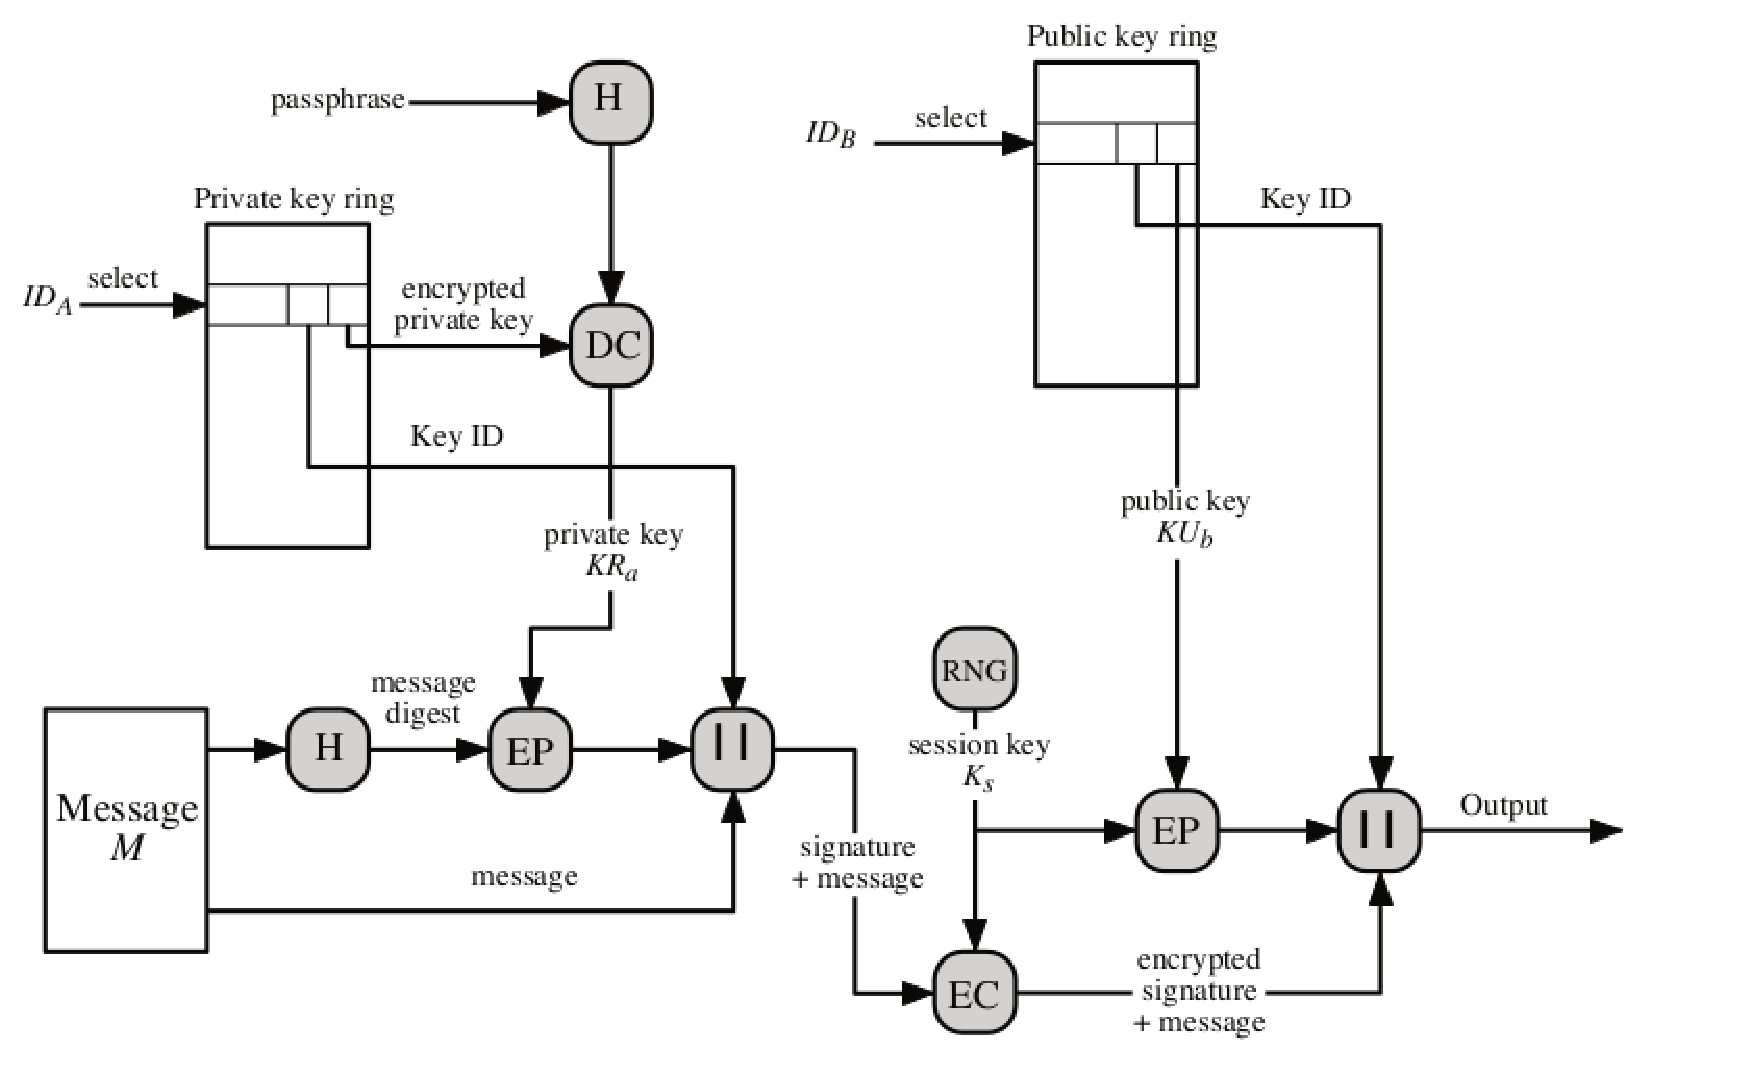
\includegraphics[width=\textwidth]{PgpMsgGen}
\end{figure}

\end{frame}

%------------------------------------------------

\begin{frame}
\frametitle{How it works}

\begin{figure}
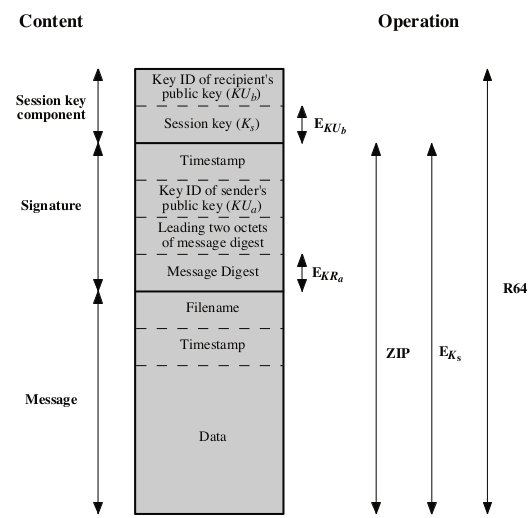
\includegraphics[scale=0.4]{PgpMsgFormat}
\end{figure}

\end{frame}

%------------------------------------------------
\section{Implementation}

\begin{frame}
\frametitle{Implementation - 1\textsuperscript{st} Iteration: Bouncy Castle API}

\begin{itemize}
\item Microsoft CryptoServiceProvider
\item SQLite for key/contacts information
\item Bouncy Castle Open Source Cryptographic functions
\end{itemize}

\end{frame}
%------------------------------------------------

\begin{frame}
\frametitle{Design}

\begin{figure}
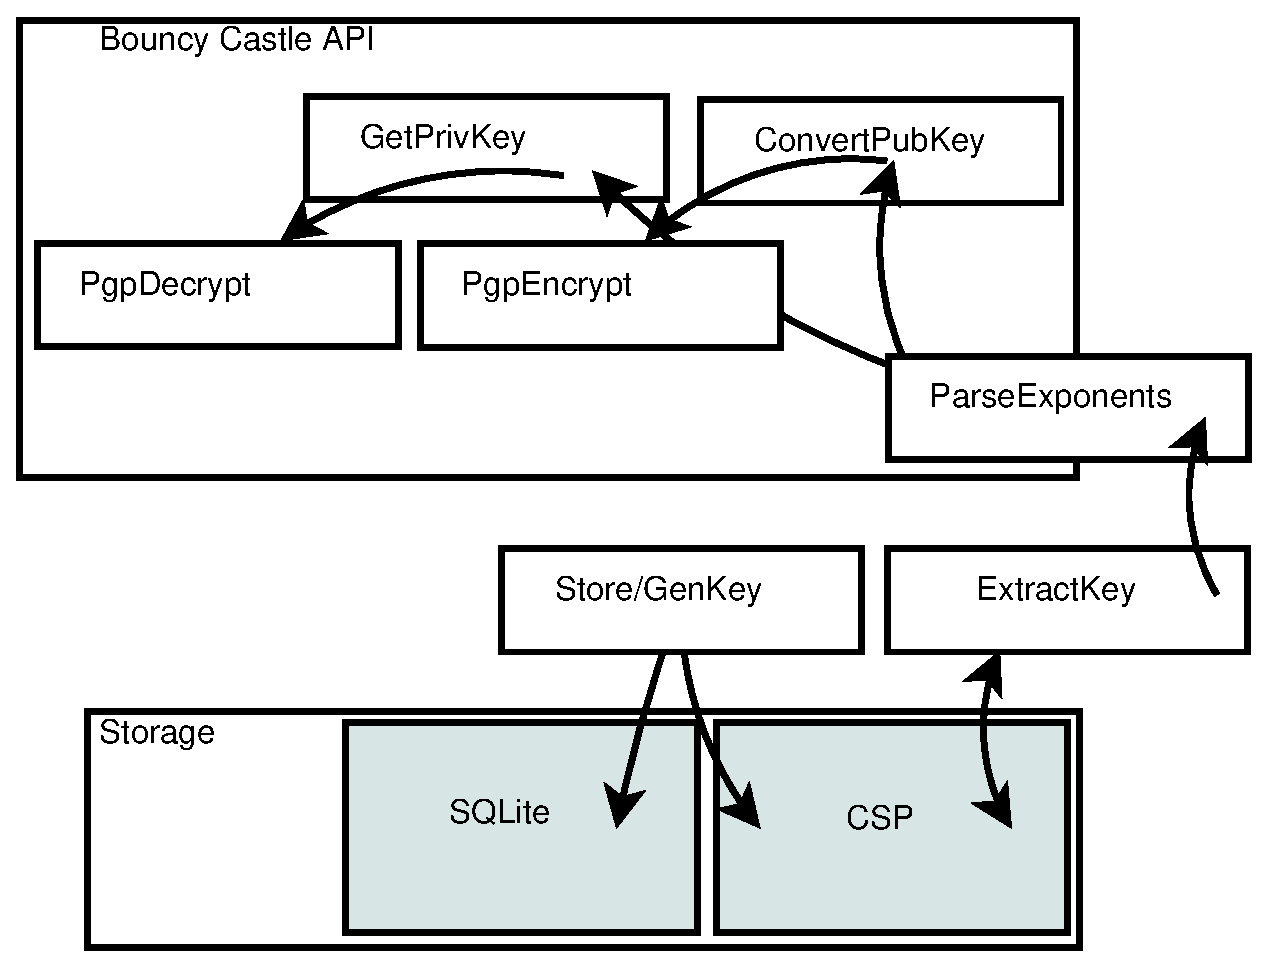
\includegraphics[scale=0.4]{Diagram1}
\end{figure}

\end{frame}

%------------------------------------------------

\begin{frame}
\frametitle{Implementation - 2\textsuperscript{nd} Iteration: Didisoft API}

\begin{itemize}
\item Didisoft's .NET API
\item Default choices: 
\begin{itemize}
\item Key Size: 2048 bits \cite{p1}
\item Asymmetric Algorithm: RSA
\item Symmetric Cipher: AES-128/CAST5
\item Hash function: SHA1, MD5, SHA256
\item Compression: ZIP
\end{itemize}
\end{itemize}

\end{frame}

%------------------------------------------------

\begin{frame}
\frametitle{Implementation - RSA vs. DSA2/ElGamal}
\begin{columns}[onlytextwidth]
\begin{column}{0.45\textwidth} % The "c" option specifies centered vertical alignment while the "t" option is used for top vertical alignment
\centering
\textbf{RSA}
\begin{itemize}
\item Integer Factorisation
\item Default in GPG \cite{wk}
\item More wide-spread
\item Faster signature verification
\item Longer signatures
\end{itemize}
\end{column}

\begin{column}{0.45\textwidth} % The "c" option specifies centered vertical alignment while the "t" option is used for top vertical alignment
\centering
\textbf{DSA2 with ElGamal}
\begin{itemize}
\item Discrete Logarithm Problem
\item Smaller signatures
\item Slightly faster signature generation
\item Shorter key length
\end{itemize}
\end{column}
\end{columns}
\end{frame}

\section{Conclusion}
\begin{frame}
\frametitle{Lessons learned}
\begin{itemize}
\item Poorly documented APIs are \emph{not good}
\item Didisoft API limitations \cite{dd}
\item Implementing OpenPGP is \emph{hard}
\end{itemize}
\end{frame}

%------------------------------------------------

\begin{frame}[fragile] % Need to use the fragile option when verbatim is used in the slide
\frametitle{Future work?}
\begin{itemize}
\item PGP/MIME support (attachments)
\item ECDSA and ECDH?
\item Advanced users configuration
\item Keccak (SHA3) \emph{vs.} MD5 or SHA1 (vulnerable \cite{sh})
\item More configurable
\end{itemize}
\end{frame}

%------------------------------------------------

\begin{frame}
\frametitle{References}
\footnotesize{
\begin{thebibliography}{99} 

\bibitem[1]{p1} Elaine Barker, Allen Roginsky (2011)
\newblock Transitions: Recommendation for Transitioning the Use of Cryptographic Algorithms and Key Lengths
\newblock \emph{NIST Special Publication 800-131A}

\bibitem[2]{dd} www.didisoft.com
\newblock OpenPGP Email messages
\newblock \emph{http://www.didisoft.com/net-openpgp/examples/openpgp-email-messages/}

\bibitem[3]{sh} Marc Stevens
\newblock Framework for MD5 \& SHA-1 Differential Path Construction and Chosen-Prefix Collisions for MD5
\newblock \emph{https://code.google.com/p/hashclash/}

\bibitem[4]{wk} Nathan Willis(June 17, 2009)
\newblock Dealing with weakness in SHA-1
\newblock \emph{http://lwn.net/Articles/337745/}

\end{thebibliography}
}
\end{frame}

%------------------------------------------------

\begin{frame}
\Huge{\centerline{Demo}}
\end{frame}

%----------------------------------------------------------------------------------------

\end{document}
